%!TEX program = xelatex
\documentclass[12pt,a4paper,utf8]{ctexart}
\usepackage{graphicx}
\usepackage{amsmath}
\usepackage{amssymb}
\usepackage{subfig}
\usepackage{cite}
\usepackage[ntheorem]{empheq}
\usepackage{enumitem}
\usepackage{fullpage}
\usepackage{cleveref}
\usepackage{cellspace}
\usepackage{listings}
\usepackage{color}
\usepackage{tasks}
\settasks{
	style=itemize,
	after-item-skip=0pt
}
\definecolor{gray}{rgb}{0.5,0.5,0.5}
\definecolor{dkgreen}{rgb}{.068,.578,.068}
\definecolor{dkpurple}{rgb}{.320,.064,.680}

% set Matlab styles
\lstset{
   language=Matlab,
   keywords={break,case,catch,continue,else,elseif,end,for,function,
      global,if,otherwise,persistent,return,switch,try,while},
   basicstyle=\ttfamily,
   keywordstyle=\color{blue}\bfseries,
   commentstyle=\color{dkgreen},
   stringstyle=\color{dkpurple},
   backgroundcolor=\color{white},
   tabsize=4,
   showspaces=false,
   showstringspaces=false
}

\begin{document}

\CJKfamily{zhkai}       


\begin{center}
\textbf{作业二}\\
\textbf{林成渊 ~~~~~ PB18051113 ~~~~~ \zhtoday}\\
\end{center}
\textit{}
\vspace{\baselineskip}

\begin{enumerate}
\item[EX1] %\textbf{重心插值公式(barycentric interpolation formula)}  
考虑以下C代码段
\begin{lstlisting}[frame=single]
	for( i = 0 ; i <= 100 ; i++ ){
		A[i] = B[i] + C;
	}
\end{lstlisting}
假定A和B是32位整数的数组,C和i是32位整数。假定所有数据值及其地址都保存在存储器中(A、B、C、i分别位于地址1000、3000、5000、7000处)。写出RISC-V代码,并计算共需要执行多少条指令?代码大小为多少?

解:实际的汇编指令根据编译器的不同、设计思路的不同而有所差异。此处仅展示手工书写的一种汇编代码方案。(此处不做代码优化,仅考虑完成当前任务,将A、B、C、i赋以正确的值)
\begin{lstlisting}[frame=single]
addi x1,x0,1750
slli x1,x1,2
addi x2,x0,1250
slli x2,x2,2
lw x2,0(x2)
addi x3,x0,1500
slli x3,x3,1
addi x5,x0,0
sw x5,0(x1)
addi x6,x0,100
L1:
slli x7,x5,2
add x8,x7,x3
lw x8,0(x8)
addi x9,x0,0
add x9,x8,x2
addi x8,x7,1000
sw x9,0(x8)
addi x5,x5,1
sw x5,0(x1)
ble x5,x6,L1
\end{lstlisting}
已使用Ripes验证其正确性。共计20条指令,需要执行$ 10+10\times 101 = 1020 $条指令。计算代码大小$ 20 \times 32 bits = 80 bytes$,共计40字节。

\item[EX2] %\textbf{重心插值公式(barycentric interpolation formula)}  
对于以下情况,考虑针对指令集体系结构的指令编码

\textbf{1.处理器的指令长度为12位,有32个通用寄存器,是否可能拥有如下指令编码?说明理由。}
\begin{itemize}
	\item 3个两地址指令
	\item 30个单地址指令
	\item 45个零地址指令
\end{itemize}

解:可行。由于有32个通用寄存器,一个寄存器的地址需要$ log_2 32 = 5 $位。此处展示一种分配方案。

首先考虑两地址指令,其寄存器地址需要$ 2 \times 5 = 10 $位,剩下的2位(标记为AB位)刚好用于标记3个两地址指令、其它指令共计4种情况。记其它指令对应的AB取值为$ ab $

再考虑单地址指令,由于AB两位中只有一种取值对应着其它指令,这时还剩下$ 12 - 2= 10 $位的空间供其与零地址指令一同分配,首先寄存器地址需要5位,剩下的5位记作CDEFG,共计$ 1\times 2^5 = 32 $种情况,其中30种提供给单地址指令,单地址指令分配完毕。剩下两种情况用于标记零地址指令,记作$cdefg_1$、$ cdefg_2 $。

最后考虑零地址指令,考虑$ AB = ab $,$ CDEFG = cdefg_1 $或$ cdefg_2 $的情况,剩下5位供其自由分配,那么留给它的可分配空间为$ 2 \times 2^5 = 64$,完全满足45个零地址指令的分配要求。

按照如上叙述的分配方案,足够为这些指令分配指令编码。故此题答案为可行。

\textbf{2.假定指令长度和地址段的大小如上所述,判断是否可能拥有如下指令编码?说明理由。}

\begin{itemize}
	\item 3个两地址指令
	\item 31个单地址指令
	\item 35个零地址指令
\end{itemize}

解:不可行。12位指令共计$ 2^{12} = 4096$种取值。3个两地址指令总共有$ 3 \times 2^5 \times 2^5  = 3072$种可能,31个单地址指令总共有$ 31 \times 2^5 = 992 $种可能,35个零地址指令有$ 35 $种可能,三种指令总共$ 3072 + 992 + 35 = 4099 $种可能,编码在12位指令里则必有两个不同指令拥有相同编码,超出了12位指令的表达上限。

\textbf{3.假定指令长度和地址段的大小如上所述,进一步假定已经拥有了3个两地址指令和24个零地址指令。最多可以为这一处理器编码多少个单地址指令。}

解:最多可以再编码31条单地址指令。12位指令共计$ 2^{12} = 4096$种取值,3个两地址指令总共有$ 3 \times 2^5 \times 2^5  = 3072$种可能,24个零地址指令有$ 24 $种可能,余下$ 4096 - 3072 - 24 = 1000 $种,则可编码的单地址指令为$ \llcorner 1000 / 2^5 \lrcorner = 31 $条。

\item[EX3] %\textbf{重心插值公式(barycentric interpolation formula)}  
一个16进制数434F4D5055544552,将其存储在64位对齐的双字中,且存储器按字节编址。内存的物理排列为从左至右,地址由低到高。

\textbf{1.用大端顺序写出要存储的值。接下来,将每个字节翻译为ASCII字符,写出存储的字符串}

答:地址由低到高存储依次为:434F4D5055544552。存储的字符串为:COMPUTER。

\textbf{2.用小端顺序写出要存储的值。将每个字节翻译为ASCII字符,写出存储的字符串}

答:地址由低到高存储依次为:52455455504D4F43。存储的字符串为:RETUPMOC。

\textbf{3.当以大端顺序存储时,可以从给定的64位双字中读取的所有非对齐2字节的十六进制数是多少?}

答:4F4D,5055,5445。

\textbf{4.当以小端顺序存储时,可以从给定的64位双字中读取的所有非对齐4字节的十六进制数是多少?}

答:4F4D5055,4D505554,50555445。

\item[EX4] %\textbf{重心插值公式(barycentric interpolation formula)}  
有一个采用单周期实现的计算机。原机器的时钟周期为7ns。在流水线分割后,测得的时间数据为:IF,1ns\ ;\ ID,1.5ns\ ;\ EX,1ns\ ;\ MEM,2ns\ ;\ WB,1.5ns。流水线寄存器的延迟为0.1ns。

\textbf{1. 5级流水化机器的时钟周期时间为多少?}

解:时钟周期时间$ T = min{\mbox{各段时间}} + \mbox{流水线寄存器延迟}  = 2ns + 0.1ns = 2.1ns$。

\textbf{2. 如果每4条指令有一次停顿,新机器的CPI是多少?}

解:新机器的CPI$  = 5 / 4 = 1.25 $。

\textbf{3. 流水化机器相对于单周期机器的加速比是多少?}

解:考虑理想情况,不需要停顿,则
\begin{equation}
	\begin{aligned}
		\mbox{加速比} &= \frac {\mbox{单周期机器CPI} \times \mbox{单周期机器时钟周期}}{\mbox{流水化机器CPI} \times  \mbox{流水化机器时钟周期}} \\
		&= \frac{1 Circ/Ins \times 7ns/Circ}{1 Circ/Ins \times 2.1ns/Circ} \\
		& \approx 3.33
	\end{aligned}\nonumber
\end{equation}
考虑(2)中每4条指令有一次停顿的情况,则
\begin{equation}
	\begin{aligned}
		\mbox{加速比} &= \frac {\mbox{单周期机器CPI} \times \mbox{单周期机器时钟周期}}{\mbox{流水化机器CPI} \times  \mbox{流水化机器时钟周期}} \\
		&= \frac{1 Circ/Ins \times 7ns/Circ}{1.25 Circ/Ins \times 2.1ns/Circ} \\
		&\approx 2.67
	\end{aligned}\nonumber
\end{equation}

\item[EX5] %\textbf{重心插值公式(barycentric interpolation formula)} 
第一台机器是5级流水线,时钟周期为1ns。第二台机器是12级流水线,时钟周期为0.6ns。由于数据相关,5级流水线每5条指令经历一次stall,而12级流水线每8条指令经历三次stall。此外,分支占全部指令的20\%,两台机器的预测错误率都是5\%。
                          
\textbf{1. 仅考虑数据相关,12级流水线相对于5级流水线的加速比为多少?}

解:5级流水线的CPI$ = (5+1) / 5  = 1.2$,12级流水线的CPI$ = (8+3) / 8 = 1.375$,所以
\begin{equation}
	\begin{aligned}
		\mbox{加速比} &= \frac{\mbox{5级流水线机器CPI} \times \mbox{5级流水线机器时钟周期}}{\mbox{12级流水线机器CPI} \times  \mbox{12级流水线机器时钟周期}} \\
		&= \frac{1.2 Circ/Ins \times 1ns/Circ}{1.375 Circ/Ins \times 0.6ns/Circ} \\
		&\approx 1.46
	\end{aligned}\nonumber
\end{equation}

\textbf{2. 在考虑分支预测错误而导致stall的情况下,如果第一台机器的分支预测错误的额外代价为2个周期,而第二台机器为5个周期,则每种机器的CPI为多少?}

解:5级流水线的CPI
\begin{equation}
	\begin{aligned}
		CPI_{5\ Stages} &= (5\times (1+20\% \times 5\% \times 2) + 1) / 5 \\
		&= 1.22
	\end{aligned}\nonumber
\end{equation}
12级流水线的CPI
\begin{equation}
	\begin{aligned}
		CPI_{12\ Stages} &= (8\times (1+20\% \times 5\% \times 5 ) + 3) / 8 \\
		&\approx 1.425
	\end{aligned}\nonumber
\end{equation}

\item[EX6] %\textbf{重心插值公式(barycentric interpolation formula)} 
有一条静态多功能流水线由5段组成,加法用1,3,4,5段,乘法用1,2,5段,第三段的时间为$ 2\Delta t $,其余各段时间均为$ \Delta t $,而且流水线的输出可以直接返回输入端或暂存于相应的流水寄存器中。现要在该流水线上计算$ \prod_{i = 1}^{4} (A_i + B_i)$,画出时空图,并计算其吞吐率、加速比和效率
\begin{figure}[htbp]
	\centering
	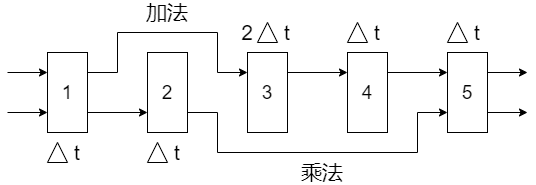
\includegraphics[width=0.7\linewidth]{EX6T}
	\caption{EX6题目示意图}
	\label{fig:ex6t}
\end{figure}


解:由题意设置为7个任务,依次执行。
\begin{tasks}(2)
	\task \textbf{1:}\quad $ C_1 = A_1 + B_1 $
	\task \textbf{2:}\quad $ C_2 = A_2 + B_2 $
	\task \textbf{3:}\quad $ C_3 = A_3 + B_3 $
	\task \textbf{4:}\quad $ C_4 = A_4 + B_4 $
	\task \textbf{5:}\quad $ D_1 = C_1 \times C_2 $ 
	\task \textbf{6:}\quad $ D_2 = C_3 \times C_4 $
	\task \textbf{7:}\quad $ D = D_1 \times D_2 $
\end{tasks}
绘图得
\begin{figure}[htbp]
	\centering
	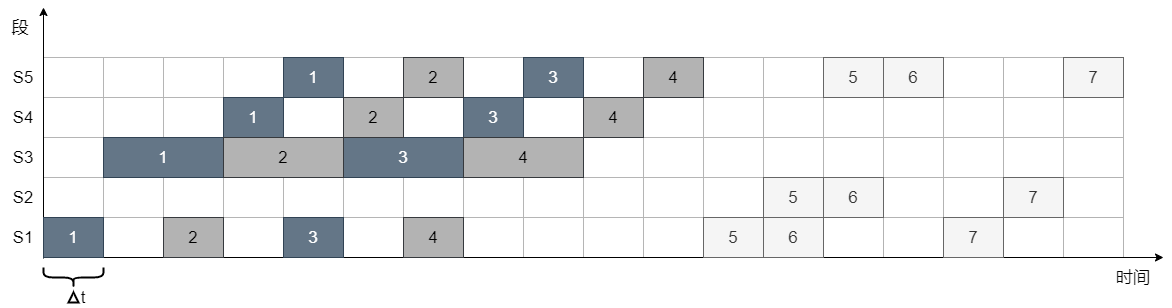
\includegraphics[width=0.9\linewidth]{EX6}
	\caption{时空图}
	\label{fig:ex6}
\end{figure}

由图算得诸指标如下,

吞吐率$ = 7/(18\Delta t) $

加速比$ =  (4 \times (1+2+1+1)\Delta t + 3\times (1+1+1)\Delta t) /(18\Delta t) \approx 1.611  $

各流水段效率:
\begin{tasks}(2)
	\task \textbf{流水段1:}\quad 效率$ e_1 = 7/18 $
	\task \textbf{流水段2:}\quad 效率$ e_2 = 3/18 $
	\task \textbf{流水段3:}\quad 效率$ e_3 = 8/18 = 4/9 $
	\task \textbf{流水段4:}\quad 效率$ e_4 = 4/18 = 2/9 $
	\task \textbf{流水段5:}\quad 效率$ e_5 = 7/18$ 
\end{tasks}
流水线总体效率
$$E = \frac{e_1+e_2+e_3+e_4+e_5}{5} = 29/90 \approx 32.22\%$$


\end{enumerate}




\end{document}
